\documentclass[10pt, letterpaper]{article}
\usepackage{amssymb}
\usepackage[utf8]{inputenc}
\usepackage{amsmath}
\usepackage[spanish]{babel}
\usepackage{tikz}
\usepackage{graphicx}
\newcommand{\N}{\mathbb{N}}
\newcommand{\R}[1]{$\mathbb{R}^#1$}
\newcommand{\Phisub}[1]{$\varphi_#1$}
\newcommand{\negrita}[1]{\textbf{#1}}
\newcommand{\integral}[2]{\int_{#1}^{#2}}
\newcommand{\limite}[2]{\lim_{#1 \to #2} }
\newcommand{\matriz}[4]{\begin{pmatrix}
#1 & #2\\
#3 & #4
\end{pmatrix}}


\providecommand{\norm}[1]{\lVert#1\rVert}
\usepackage{amsthm}
\usepackage{pgfplots}
\usepackage{mathtools}

\newtheorem{definition}{Definición}[section]
\newtheorem{observation}{Observación}[section]
\newtheorem{theorem}{Teorema}[section]
\newtheorem{proposition}{Proposición}[section]
\newtheorem{lemma}{Lema}[section]
\newtheorem{corollary}{Corolario}[section]
\newtheorem{example}{Ejemplo}[section]
\newtheorem{exercise}{Ejercicio}[section]



\title{	

	\normalfont\normalsize
	\textsc{Universidad de Murcia}\\ 
	\vspace{25pt} % Whitespace
	\rule{\linewidth}{0.5pt} % Thin top horizontal rule
	\vspace{20pt}\\ % Dará error hasta que escribas algo en el título
	{\huge Apuntes Física
}\\ % The assignment title
	\vspace{12pt} % Whitespace
	\rule{\linewidth}{2pt}\\ % Thick bottom horizontal rule
	\vspace{12pt} % Whitespace
	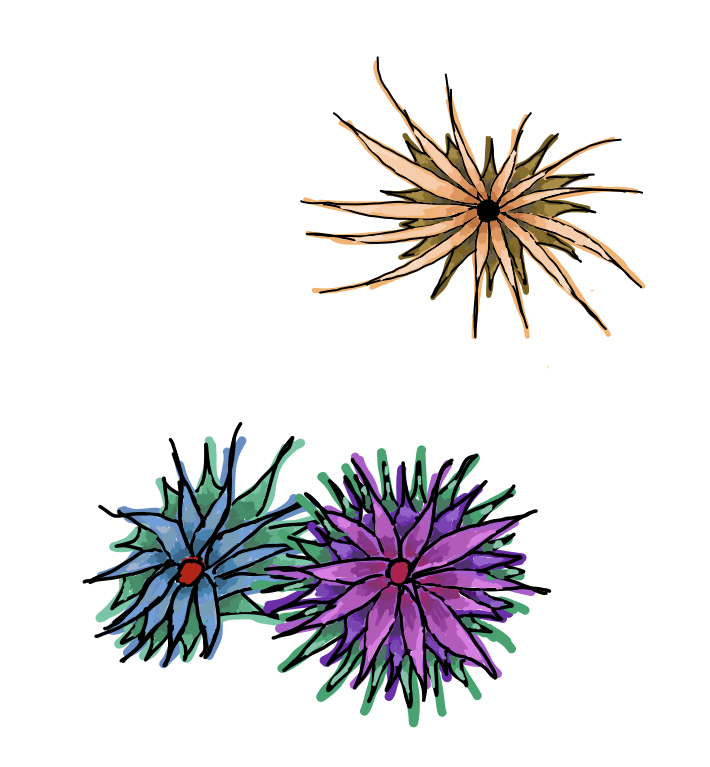
\includegraphics[scale=0.25]{floresportada.png}
}


\author{\LARGE Alonso Oma Alonso} % Your name

  
 
\date{\normalsize\today} % Today's date (\today) or a custom date



\begin{document}

\begin{titlepage}
	\maketitle
\end{titlepage}

\newpage
\tableofcontents
\newpage

\begin{section} {Cálculo vectorial}
    \begin{definition}
        Una funcióncontinua $\vec{\alpha}:\left[a, b\right] \Rightarrow \mathbb{R}^n$ se denomina un camino (trayectoria, path) en $\mathbb{R}^n$. La imagen de $\vec{\alpha}$ se denomina curva.
    \end{definition}

    \begin{example}
        Curva =: $\{(x,y) \in \mathbb{R}^n: x^2 + y^2 = 4\}$

        \negrita{Caminos:}

        \[\begin{matrix}
            \vec{\alpha_1}: \left[0, 2\pi \right] \rightarrow \mathbb{R}^2 \\
            \vec{\alpha_1}(\theta) = (2cos(\theta), 2sen(\theta))
        \end{matrix}\]

    \end{example}
\end{section}

\end{document}